\paragraph{QuizziPedia::Front-End::ModelViews::QuestionsModelView}
			
			\label{QuizziPedia::Front-End::ModelViews::QuestionsModelView}
			
			\begin{figure}[ht]
				\centering
				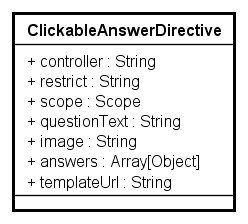
\includegraphics[scale=0.5,keepaspectratio]{UML/Classi/Front-End/QuizziPedia_Front-end_Templates_ClickableAnswerTemplate.png}
				\caption{QuizziPedia::Front-End::ModelViews::QuestionsModelView}
			\end{figure} \FloatBarrier
			
			\begin{itemize}
				\item \textbf{Descrizione}: classe di tipo modelview la cui istanziazione è contenuta all'interno della variabile di ambiente \$scope di \textit{Angular.js\ped{G}}. All'interno di essa sono presenti le variabili e i metodi necessari per il \textit{Two-Way Data-Binding\ped{G}} tra le directive che compongono dinamicamente la vista della domanda e il controller \texttt{QuestionsController};
				\item \textbf{Utilizzo}: viene utilizzata per effettuare il \textit{Two-Way Data-Binding\ped{G}} tra le directive che compongono dinamicamente la vista della domanda e il controller \texttt{QuestionsController} rendendo disponibili variabili e metodi;
				\item \textbf{Relazioni con altre classi}: 
				\begin{itemize} 
					\item \textit{OUT} \texttt{QuestionsController}: questa classe permette di gestire il recupero delle domande per poterle stampare nella modalità allenamento;
					\item \textit{OUT} \texttt{ClickableAnswerDirective}: rappresenta il componente grafico che permette all'utente di visualizzare la domanda ad area cliccabile nell'immagine. Viene visualizzato dinamicamente all'interno delle views TrainingView e FillingQuestionnaireView mediante il controller QuestionsController;
					\item \textit{OUT} \texttt{EmptySpaceAnswerDirective}: rappresenta il componente grafico che permette all'utente di visualizzare l'esercizio a riempimento di spazi vuoti. Viene visualizzato dinamicamente all'interno delle views TrainingView e FillingQuestionnaireView mediante il controller QuestionsController;
					\item \textit{OUT} \texttt{HeaderTextQuestionDirective}: rappresenta il componente grafico che presenta all'utente il testo della domanda, l'argomento e le parole chiave. Viene visualizzato dinamicamente all'interno delle views TrainingView e FillingQuestionnaireView mediante il controller QuestionsController;
					\item \textit{OUT} \texttt{LinkingAnswerDirective}: rappresenta il componente grafico che permette all'utente di visualizzare la domanda di collegamento. Viene visualizzato dinamicamente all'interno delle views TrainingView e FillingQuestionnaireView mediante il controller QuestionsController;
					\item \textit{OUT} \texttt{MultipleChoiceAnswerDirective}: rappresenta il componente grafico che permette all'utente di visualizzare la domanda a risposta multipla. Viene visualizzato dinamicamente all'interno delle views TrainingView e FillingQuestionnaireView mediante il controller QuestionsController;
					\item \textit{OUT} \texttt{SortImagesAnswerDirective}: rappresenta il componente grafico che permette all'utente di visualizzare la domanda ad ordinamento di immagini. Viene visualizzato dinamicamente all'interno delle views TrainingView e FillingQuestionnaireView mediante il controller QuestionsController;
					\item \textit{OUT} \texttt{SortTextAnswerDirective}: rappresenta il componente grafico che permette all'utente di visualizzare la domanda ad ordinamento di stringhe. Viene visualizzato dinamicamente all'interno delle views TrainingView e FillingQuestionnaireView mediante il controller QuestionsController;
					\item \textit{OUT} \texttt{TrainingSetUpDirective}: rappresenta il componente grafico che permette all'utente di selezionare l'argomento e le parole chiave per iniziare un allenamento con queste caratteristiche. Viene visualizzato dinamicamente all'interno della view TrainingView mediante il controller TrainingController;
					\item \textit{OUT} \texttt{TrueFalseAnswareDirective}: rappresenta il componente grafico che permette all'utente di visualizzare la domanda vero e falso. Viene visualizzato dinamicamente all'interno delle views TrainingView e FillingQuestionnaireView mediante il controller QuestionsController;					
				\end{itemize}
				\item \textbf{Attributi}: 
				\begin{itemize}
					\item \texttt{+ piecesOfQuestion: Array[Object]} \\
					Questo attributo è un \texttt{array} di \texttt{Object} contenente la domanda da visualizzare dinamicamente attraverso le direttive all'interno le direttive di allenamento e di compilazione dei questionari;
					\item \texttt{+ objAnswer: Array[Object]} \\
					Questo attributo è un \texttt{array} di \texttt{Object} contenente le risposte date fino a quel momento dall'utente in una domanda. L'\texttt{Object} è così formato: \\
					\begin{itemize}
						\item \texttt{+ typeQuestion: String} \\
						Questo attributo rappresenta il tipo della domanda;
						\item \texttt{+ answerGiven: Array[String]} \\
						Questo attributo rappresenta le riposte scelta dall'utente fino a quel momento.
					\end{itemize}
				\end{itemize}
				\item \textbf{Metodi}: 
				\begin{itemize}
					\item \texttt{+} \texttt{addAnswer(index: Number, typeQuestion: String, answerGiven: Array[String]): void} \\
					Metodo che gestisce l'evento di selezione delle risposte. \\
					\textbf{Parametri}:
					\begin{itemize}
						\item \texttt{index: Number} \\
						Parametro contenente l'indice della risposta di cui si vuole tenere traccia. Rappresenta anche l'indice dell'\texttt{array objAswer} in cui verrà inserito l'oggetto delle risposte date;
						\item \texttt{typeQuestion: String} \\
						Parametro contenente una stringa la quale indica la tipologia della domanda;
						\item \texttt{answerGiven: Array[String]} \\
						Parametro contenente l'array di risposte date dall'utente aggiornato all'ultima iterazione;
					\end{itemize};
					\item \texttt{+} \texttt{answerGiven(index: Number): Array[String]} \\
					Metodo di supporto che ritorna un \texttt{array} di stringhe contenente le risposte date. Si occupa di recuperare le risposte date nelle domande vero/falso, risposta multipla e ad area cliccabile.\\
					\textbf{Parametri}:
					\begin{itemize}
						\item \texttt{index: Number} \\
						Parametro contenente l'indice della risposta di cui si vuole raccogliere le risposte date; 
					\end{itemize}
					\item \texttt{+} \texttt{orderChosen(index: Number): Array[String]} \\
					Metodo di supporto che ritorna un \texttt{array} di stringhe contenente le risposte date. Si occupa di recuperare le risposte date nelle domande ad ordinamento e di riempimento di spazi.\\
					\textbf{Parametri}:
					\begin{itemize}
						\item \texttt{index: Number} \\
						Parametro contenente l'indice della risposta di cui si vuole raccogliere le risposte date; 
					\end{itemize}
					\item \texttt{+} \texttt{linkingMade(index: Number): Array[String]} \\
					Metodo di supporto che ritorna un \texttt{array} di stringhe contenente le risposte date. Si occupa di recuperare le risposte date nelle domande a collegamento.\\
					\textbf{Parametri}:
					\begin{itemize}
						\item \texttt{index: Number} \\
						Parametro contenente l'indice della risposta di cui si vuole raccogliere le risposte date; 
					\end{itemize}
					\item \texttt{+} \texttt{loadNewQuestionBy(topic: String, keywords: Array[String], level: Number): void} \\
					Metodo che gestisce l'evento per scaricare una nuova domanda in base ai parametri passati. \\
					\textbf{Parametri}:
					\begin{itemize}
						\item \texttt{topic: String} \\
						Parametro contenente l'argomento della domanda;
						\item \texttt{keywords: Array[String]} \\
						Parametro contenente un\texttt{array} di stringhe che rappresenta le keywords scelte per l'allenamento;
						\item \texttt{level: Number} \\
						Parametro contenente il livello dell'utente;
					\end{itemize}
					\item \texttt{+} \texttt{loadNewQuestion(question: QuestionItemModel): void} \\
					Metodo che gestisce l'evento per visualizzare una nuova domanda. \\
					\textbf{Parametri}:
					\begin{itemize}
						\item \texttt{question: QuestionItemModel} \\
						Parametro contenente un riferimento all'oggetto di tipo \texttt{QuestionItemModel};
					\end{itemize}
					\item \texttt{+} \texttt{checkAnswer(): boolean} \\ 
					Metodo che controlla che le risposte date siano corrette;
				\end{itemize}
			\end{itemize}
			
				